\documentclass{article}
\usepackage{amssymb}
\usepackage{graphicx} % Required for inserting images
\usepackage{float}
\usepackage{ctex}
\usepackage{enumitem}
\usepackage{amsmath} 
\usepackage[a4paper, margin=1in]{geometry}
\usepackage{xcolor}
\title{普通物理}
\author{Zhang}


\begin{document}

\maketitle
\textcolor{magenta}{\textbf{已经过检查的题目,其序号将以洋红色标记。}}
\section*{2020}

\subsection*{\textcolor{magenta}{1.1}}

终极速度推导:
\subsubsection*{已知条件}
\begin{itemize}
  \item 质点质量:\( m \)
  \item 重力加速度:\( g \)
  \item 空气阻力:\( f = -\gamma v \)(阻力方向与速度方向相反)
\end{itemize}

\subsubsection*{动力学方程建立}
根据牛顿第二定律:
\[
m\frac{dv}{dt} = mg - \gamma v
\]

\subsubsection*{终极速度条件}
当加速度为零时(\( \frac{dv}{dt} = 0 \)),达到受力平衡:
\[
0 = mg - \gamma v_{\text{terminal}}
\]

\subsubsection*{终极速度解}
解得:
\[
v_{\text{terminal}} = \frac{mg}{\gamma}
\]

\subsubsection*{完整微分方程验证}
将方程改写为:
\[
\frac{dv}{dt} = g - \frac{\gamma}{m}v
\]

分离变量并积分:
\[
\int_0^{v}\frac{dv'}{g - \frac{\gamma}{m}v'} = \int_0^{t}dt'
\]

解得速度随时间变化规律:
\[
v(t) = \frac{mg}{\gamma}\left(1 - e^{-\frac{\gamma}{m}t}\right)
\]

当\( t \to \infty \)时,指数项衰减至零,最终得到:
\[
\boxed{v_{\text{terminal}} = \dfrac{mg}{\gamma}}
\]

\subsection*{1.2:细杆转动分析}
\subsubsection*{已知参数}
\begin{itemize}
  \item 杆质量:\( m \)
  \item 杆长:\( L \)
  \item 转动角度:\( \theta = 60^\circ \)
\end{itemize}

\subsubsection*{角加速度计算}
\begin{align*}
  & \text{转动惯量:} I = \frac{1}{3}mL^2 \\
  & \text{重力矩:} \tau = mg\cdot\frac{L}{2}\sin\theta \\
  & \text{转动定律:} \tau = I\alpha \Rightarrow \alpha = \frac{3g}{2L}\sin\theta \\
  & \theta=60^\circ \Rightarrow \boxed{\alpha = \dfrac{3\sqrt{3}g}{4L}}
\end{align*}

\subsubsection*{角速度推导}
\begin{align*}
  & \text{能量守恒:} mg\frac{L}{2} = \frac{1}{2}I\omega^2 + mg\frac{L}{2}(1-\cos\theta) \\
  & \Rightarrow \omega = \sqrt{\frac{3g}{L}(1-\cos\theta)} \\
  & \theta=60^\circ \Rightarrow \boxed{\omega = \sqrt{\dfrac{3g}{2L}}}
\end{align*}

\subsubsection*{验证说明}
\begin{itemize}
  \item 转动惯量公式验证:使用平行轴定理确认端点转动惯量
  \item 能量守恒验证:铰链约束力不做功,仅有保守力作用
  \item 角度换算:\( 60^\circ = \dfrac{\pi}{3} \, \text{rad} \)
\end{itemize}


\subsection*{1.3}
已知条件
\begin{itemize}
    \item 膜厚:\( d = 0.55 \, \mu\text{m} = 550 \, \text{nm} \)
    \item 折射率:\( n = 1.35 \)
    \item 波长范围:\( 400 \, \text{nm} \leq \lambda \leq 700 \, \text{nm} \)
\end{itemize}

干涉条件分析
\[
\Delta = 2nd\cos\theta + \frac{\lambda}{2} \quad (\theta = 0^\circ \Rightarrow \cos\theta = 1)
\]

\subsubsection*{相长干涉条件(明纹)}
\[
2nd + \frac{\lambda}{2} = m\lambda \quad \Rightarrow \quad \lambda = \frac{2nd}{m - \frac{1}{2}}
\]
代入数据:
\[
\lambda = \frac{2 \times 1.35 \times 550}{m - 0.5} = \frac{1485}{m - 0.5} \, \text{nm}
\]

\subsubsection*{相消干涉条件(暗纹)}
\[
2nd + \frac{\lambda}{2} = \left(m + \frac{1}{2}\right)\lambda \quad \Rightarrow \quad \lambda = \frac{2nd}{m}
\]
代入数据:
\[
\lambda = \frac{1485}{m} \, \text{nm}
\]

计算结果
\subsubsection*{相长干涉波长}
\[
\begin{aligned}
m = 3: & \quad \lambda = \frac{1485}{2.5} = 594 \, \text{nm} \\
m = 4: & \quad \lambda = \frac{1485}{3.5} \approx 424.3 \, \text{nm}
\end{aligned}
\]

\subsubsection*{相消干涉波长}
\[
m = 3: \quad \lambda = \frac{1485}{3} = 495 \, \text{nm}
\]

最终答案
反射光中:
\[
\boxed{\text{波长为 } 594 \, \text{nm} \text{ 和 } 424 \, \text{nm} \text{ 的光干涉增强,波长为 } 495 \, \text{nm} \text{ 的光干涉相消}}
\]

%
\subsection*{1.4}

\subsubsection*{关键分析}
\begin{itemize}
\item \textbf{自然光通过第一个偏振片}:自然光的强度\(I_0\)被过滤为线偏振光,强度降为\(\frac{I_0}{2}\)(马吕斯定律中,自然光通过偏振片后强度保留50\%)。
\item \textbf{第二个偏振片的作用}:透射光强度由两偏振片的夹角决定,遵循马吕斯定律:
\[
I = \frac{I_0}{2} \cos^2\theta
\]
其中\(\theta\)为两偏振片的偏振方向夹角。
\end{itemize}

\subsubsection*{公式推导}
\begin{enumerate}
\item \textbf{转动前}(夹角为\(\alpha_1\)):
\[
I_1 = \frac{I_0}{2} \cos^2\alpha_1
\]
\item \textbf{转动后}(夹角为\(\alpha_2\)):
\[
I_2 = \frac{I_0}{2} \cos^2\alpha_2
\]
\item \textbf{强度比值}:
\[
\frac{I_2}{I_1} = \frac{\frac{I_0}{2} \cos^2\alpha_2}{\frac{I_0}{2} \cos^2\alpha_1} = \frac{\cos^2\alpha_2}{\cos^2\alpha_1}
\]
\end{enumerate}

最终答案
转动{\color{red}后前}透射光强度之比为:
\[
\boxed{\frac{\cos^2\alpha_2}{\cos^2\alpha_1}}
\]

\paragraph*{说明}:
\begin{itemize}
\item 若\(\alpha_2 < \alpha_1\),则\(\cos^2\alpha_2 > \cos^2\alpha_1\),透射光强度增强。
\item 当两偏振片平行(\(\alpha = 0^\circ\))时,透射光强度最大;垂直(\(\alpha = 90^\circ\))时,透射光强度为零。
\end{itemize}
%



\subsection*{1.5}
{\color{red}不对}
\begin{enumerate}
  \item 电容器储能公式:
  \[
  W = \frac{1}{2}CU^2 = \frac{1}{2} \left( \frac{\varepsilon_0 S}{d} \right) U^2
  \]
  
  \item 相互作用力计算(能量对极板间距求导):
  \[
  F = -\frac{\partial W}{\partial d} = \frac{\varepsilon_0 S U^2}{2d^2}
  \]
  
  \item 电场应力法验证:
  \[
  \text{电场强度} \ E = \frac{U}{d},\quad \text{面电荷密度} \ \sigma = \varepsilon_0 E
  \]
  \[
  F = \frac{\sigma^2 S}{2\varepsilon_0} = \frac{\varepsilon_0 S U^2}{2d^2}
  \]
\end{enumerate}

\subsubsection*{最终答案}
\[
\boxed{F = \dfrac{\varepsilon_0 S U^2}{2d^2}}
\]

\subsection*{1.6}

\subsubsection*{电势计算}
设坐标系原点O在AB中点:
\begin{itemize}
  \item A点坐标:\( (-r, 0) \),带电荷\( +q \)
  \item B点坐标:\( (r, 0) \),带电荷\( -q \)
  \item D点坐标:\( (2r, 0) \)(位于B点外侧延长线上)
\end{itemize}

O点电势
\[
V_O = \frac{kq}{r} + \frac{k(-q)}{r} = 0
\]

{D点电势
\[
V_D = \frac{kq}{3r} + \frac{k(-q)}{r} = -\frac{2kq}{3r}
\]

\subsubsection*{功的计算}
\begin{enumerate}
  \item \textbf{O到D的功}:
  \[
  W_{O→D} = q_0(V_O - V_D) = q_0\left(0 - \left(-\frac{2kq}{3r}\right)\right) = \frac{2k q q_0}{3r}
  \]
  
  \item \textbf{D到无穷远的功}:
  \[
  W_{D→∞} = q_0(V_D - 0) = -\frac{2k q q_0}{3r}
  \]
\end{enumerate}

\subsubsection*{最终答案}
\[
\boxed{\dfrac{2k q q_0}{3r}} \quad ; \quad \boxed{-\dfrac{2k q q_0}{3r}}
\]

\subsection*{1.7 混合气体平衡温度计算}


\subsubsection*{核心公式推导}
混合过程遵循\textbf{能量守恒},总内能保持不变:
\begin{align*}
    U_{\text{总初始}} &= U_{\text{H2初始}} + U_{\text{He初始}} \\
    &= U_{\text{H2终}} + U_{\text{He终}}
\end{align*}

\subsubsection*{内能表达式}
\begin{itemize}
    \item \textbf{氢气(H₂)}:双原子分子,考虑平动和转动自由度
    \[
        U_{\text{H2}} = \frac{5}{2}nRT
    \]
    
    \item \textbf{氦气(He)}:单原子分子
    \[
        U_{\text{He}} = \frac{3}{2}nRT
    \]
\end{itemize}

\subsubsection*{能量守恒方程}
\begin{align*}
    \text{初始总内能} &: \frac{5}{2}RT_1 + \frac{3}{2}RT_2 \\
    \text{终态总内能} &: \frac{5}{2}RT + \frac{3}{2}RT = 4RT \\
    \frac{5}{2}T_1 + \frac{3}{2}T_2 &= 4T \\
    T &= \boxed{\frac{5T_1 + 3T_2}{8}}
\end{align*}

\subsubsection*{关键假设}
\begin{itemize}
    \item 氢气按刚性双原子处理(5个自由度)
    \item 氦气按单原子处理(3个自由度)
    \item 理想气体行为,无相变和化学反应
    \item 绝热系统($\Delta Q = 0$)
\end{itemize}


\subsection*{1.8 麦克斯韦速率分布曲线分析}

\subsubsection*{核心公式}
{\color{red}分析没错,答案反了}

最概然速率公式:
\[
v_p = \sqrt{\frac{2kT}{m}} = \sqrt{\frac{2RT}{\mu}}
\]

其中:
\begin{itemize}
    \item \(k\):玻尔兹曼常数
    \item \(R\):气体常数
    \item \(\mu\):摩尔质量
    \item \(T\):温度
\end{itemize}

\subsubsection*{曲线特征规律}

\noindent 曲线变化规律:
\begin{itemize}
    \item 温度升高时:
    \begin{itemize}
        \item 最概然速率\(v_p\)增大 \(\Rightarrow\) 峰位右移
        \item 分布曲线展宽 \(\Rightarrow\) 峰高降低
    \end{itemize}
    
    \item 同温度下比较不同气体:
    \begin{itemize}
        \item 摩尔质量\(\mu\)大的气体:
        \begin{itemize}
            \item \(v_p\)较小 \(\Rightarrow\) 峰位左移
            \item 分布集中 \(\Rightarrow\) 峰高增加
        \end{itemize}
    \end{itemize}
\end{itemize}

\subsubsection*{问题解析}
\begin{enumerate}
    \item \textbf{温度比较}:
    \begin{align*}
        T_1 &> T_2 \quad \text{(对应曲线(1)和(2))} \\
        \because \frac{v_{p1}}{v_{p2}} &= \sqrt{\frac{T_1}{T_2}} \\
        \text{曲线(1)峰位更靠右} &\Rightarrow T_1 > T_2
    \end{align*}
    
    \item \textbf{气体种类判别}:
    \begin{align*}
        \frac{v_{p,\text{H2}}}{v_{p,\text{O2}}} &= \sqrt{\frac{\mu_{\text{O2}}}{\mu_{\text{H2}}}} \\
        &= \sqrt{\frac{32}{2}} = 4 \\
        \text{氢气峰位更靠右} &\Rightarrow \text{曲线(1): H₂;曲线(2): O₂}
    \end{align*}
\end{enumerate}

\subsubsection*{最终结论}
\begin{itemize}
    \item 温度较高的曲线:\boxed{(1)}
    \item 氧气对应的曲线:\boxed{(2)}
\end{itemize}


\subsection*{2.1}

\begin{figure}[H]
    \centering
    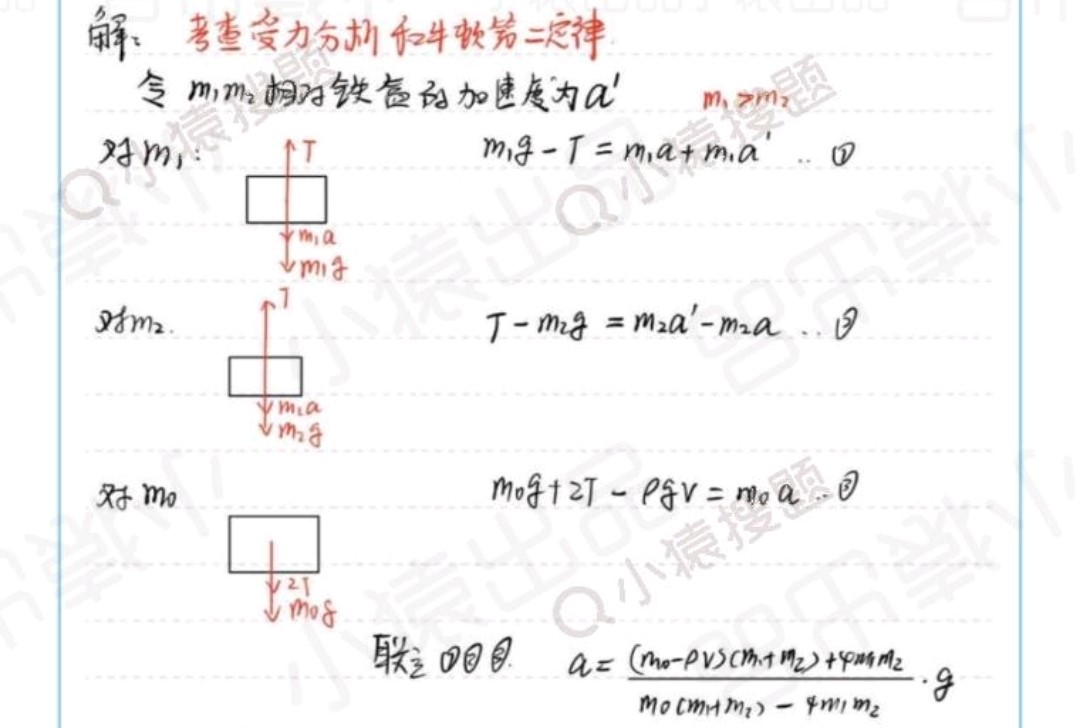
\includegraphics[width=1\linewidth]{微信图片_20250416153242.jpg}
\end{figure}


\subsection*{2.2}

\subsubsection*{对于第(1)问感应电荷分布的解答如下:}

导体球A的感应电荷分布满足以下条件:
\begin{enumerate}
    \item \textbf{内表面感应电荷}  \\
    根据导体静电平衡条件,导体内部电场为零。取半径为 \( R_b < r < R \) 的高斯面(位于导体内部),由高斯定理:
    \[
    \oint \mathbf{E} \cdot d\mathbf{A} = \frac{q_{\text{enc}}}{\epsilon_0} = 0
    \]
    高斯面内包围的电荷包括空腔中的 \( q_B \) 和导体球A内表面的感应电荷 \( q_{\text{内}} \),因此:
    \[
    q_B + q_{\text{内}} = 0 \implies q_{\text{内}} = -q_B
    \]
    \textbf{结论}:导体球A的内表面均匀分布感应电荷 \( -q_B \)。

    \item \textbf{外表面感应电荷}  \\
    导体球A原本不带电,根据电荷守恒,内表面感应出 \( -q_B \),则外表面需感应出等量异号电荷以保持整体电中性:
    \[
    q_{\text{外}} = +q_B
    \]
    \textbf{结论}:导体球A的外表面均匀分布感应电荷 \( +q_B \)。

    \item \textbf{总结分布}  \\
    感应电荷仅分布在导体表面:  
    \begin{itemize}
        \item 内表面电荷密度:\( \sigma_{\text{内}} = -\frac{q_B}{4\pi R_b^2} \)  
        \item 外表面电荷密度:\( \sigma_{\text{外}} = +\frac{q_B}{4\pi R^2} \)
    \end{itemize}
\end{enumerate}

\textbf{示意图验证}:  \\
由于空腔B与导体球A同心,电荷分布具有球对称性,内、外表面的感应电荷均呈均匀分布。

---

\textbf{最终答案}  \\
感应电荷分布为:  
\[
\boxed{
\begin{cases}
\text{导体球A内表面:均匀分布电荷 } -q_B \\
\text{导体球A外表面:均匀分布电荷 } +q_B
\end{cases}
}
\]

\subsubsection*{对于第(2)问电场和电势分布的解答如下:}




一、电场分布(按区域分析)

\begin{enumerate}
    \item \textbf{空腔内部} (\(r < R_b\))  \\
    仅受点电荷 \(q_B\) 影响,由高斯定理可得:
    \[
    \mathbf{E}_\text{内}(r) = \frac{1}{4\pi\varepsilon_0} \frac{q_B}{r^2} \mathbf{e}_r
    \]
    \textbf{方向}:沿径向向外。

    \item \textbf{导体内部} (\(R_b \leq r \leq R\))  \\
    导体处于静电平衡状态,内部电场为零:
    \[
    \mathbf{E}_\text{导体}(r) = 0
    \]

    \item \textbf{导体外部} (\(r > R\))  \\
    等效于外表面电荷 \(+q_B\) 集中在球心产生的电场:
    \[
    \mathbf{E}_\text{外}(r) = \frac{1}{4\pi\varepsilon_0} \frac{q_B}{r^2} \mathbf{e}_r
    \]
    \textbf{方向}:沿径向向外。
\end{enumerate}



二、电势分布(取无穷远为零势点)

\begin{enumerate}
    \item \textbf{空腔内部} (\(r < R_b\))  \\
    电势由 \(q_B\)、内表面感应电荷 \(-q_B\) 和外表面电荷 \(+q_B\) 共同贡献:
    \[
    V_\text{内}(r) = \frac{1}{4\pi\varepsilon_0} \left( \frac{q_B}{r} - \frac{q_B}{R_b} + \frac{q_B}{R} \right)
    \]
    \textbf{简化}:
    \[
    V_\text{内}(r) = \frac{1}{4\pi\varepsilon_0} \left( \frac{q_B}{r} + q_B \left( \frac{1}{R} - \frac{1}{R_b} \right) \right)
    \]

    \item \textbf{导体内部} (\(R_b \leq r \leq R\))  \\
    导体为等势体,电势等于外表面电势:
    \[
    V_\text{导体} = \frac{1}{4\pi\varepsilon_0} \frac{q_B}{R}
    \]

    \item \textbf{导体外部} (\(r > R\))  \\
    仅由外表面电荷 \(+q_B\) 贡献:
    \[
    V_\text{外}(r) = \frac{1}{4\pi\varepsilon_0} \frac{q_B}{r}
    \]
\end{enumerate}



三、连续性验证

\begin{itemize}
    \item 在 \(r = R_b\) 处:  
    \[
    V_\text{内}(R_b) = \frac{1}{4\pi\varepsilon_0} \frac{q_B}{R} = V_\text{导体}
    \]
    \item 在 \(r = R\) 处:  
    \[
    V_\text{导体} = \frac{1}{4\pi\varepsilon_0} \frac{q_B}{R} = V_\text{外}(R)
    \]
    电势连续,符合物理规律。
\end{itemize}



最终答案

\textbf{电场分布}:
\[
\boxed{
\mathbf{E}(r) = 
\begin{cases}
\displaystyle \frac{q_B}{4\pi\varepsilon_0 r^2} \mathbf{e}_r, & r < R_b \\
0, & R_b \leq r \leq R \\
\displaystyle \frac{q_B}{4\pi\varepsilon_0 r^2} \mathbf{e}_r, & r > R
\end{cases}
}
\]

\textbf{电势分布}:
\[
\boxed{
V(r) = 
\begin{cases}
\displaystyle \frac{q_B}{4\pi\varepsilon_0} \left( \frac{1}{r} + \frac{1}{R} - \frac{1}{R_b} \right), & r < R_b \\
\displaystyle \frac{q_B}{4\pi\varepsilon_0 R}, & R_b \leq r \leq R \\
\displaystyle \frac{q_B}{4\pi\varepsilon_0 r}, & r > R
\end{cases}
}
\]

\subsubsection*{对于第(3)问(空腔B与导体球A不同心)的解答如下:}

{\color{red}不对}
\paragraph*{一、感应电荷分布}


\begin{enumerate}
    \item \textbf{内表面感应电荷}  \\
    • \textbf{总电荷量}:仍为 \(-q_B\)(由高斯定理保证,与空腔位置无关)。  \\
    • \textbf{分布特性}:因空腔偏离中心,内表面电荷分布\textbf{不再均匀}。电荷密度与空腔几何位置相关,在靠近点电荷 \(q_B\) 的一侧密度更高。  \\
    • \textbf{数学描述}:  \\
    \[
    \sigma_{\text{内}}(\theta, \phi) \neq \text{常数}, \quad \oint_{\text{内表面}} \sigma_{\text{内}} \, dA = -q_B
    \]

    \item \textbf{外表面感应电荷}  \\
    • \textbf{总电荷量}:仍为 \(+q_B\)(由电荷守恒定律保证)。  \\
    • \textbf{分布特性}:\textbf{均匀分布}。导体球A为孤立导体,外表面电荷为保持等势体,自动调整至均匀分布。  \\
    \[
    \sigma_{\text{外}} = \frac{q_B}{4\pi R^2}
    \]
\end{enumerate}


\paragraph*{二、电场分布}


\begin{enumerate}
    \item \textbf{空腔内部} (\(r < R_b\))  \\
    • 电场由 \(q_B\) 和内表面感应电荷共同产生,由于内表面电荷分布不均匀,\textbf{电场失去球对称性},方向与大小随空间变化:  
    \[
    \mathbf{E}_\text{内}(r, \theta, \phi) \neq \frac{q_B}{4\pi\varepsilon_0 r^2} \mathbf{e}_r
    \]

    \item \textbf{导体内部} (\(R_b \leq r \leq R\))  \\
    • 导体静电平衡时内部电场仍为零:  
    \[
    \mathbf{E}_\text{导体} = 0
    \]

    \item \textbf{导体外部} (\(r > R\))  \\
    • 电场由外表面均匀分布的 \(+q_B\) 产生,等效于球心处点电荷的电场,\textbf{保持球对称性}:  
    \[
    \mathbf{E}_\text{外}(r) = \frac{1}{4\pi\varepsilon_0} \frac{q_B}{r^2} \mathbf{e}_r
    \]
\end{enumerate}



\paragraph*{三、电势分布}

\begin{enumerate}
    \item \textbf{空腔内部} (\(r < R_b\))  \\
    • 电势为常数,与导体球A的电势相等(因导体为等势体):  
    \[
    V_\text{内} = \frac{1}{4\pi\varepsilon_0} \frac{q_B}{R}
    \]

    \item \textbf{导体内部} (\(R_b \leq r \leq R\))  \\
    • 电势与空腔内部相同:  
    \[
    V_\text{导体} = \frac{1}{4\pi\varepsilon_0} \frac{q_B}{R}
    \]

    \item \textbf{导体外部} (\(r > R\))  \\
    • 电势由外表面电荷决定,与同心情况一致:  
    \[
    V_\text{外}(r) = \frac{1}{4\pi\varepsilon_0} \frac{q_B}{r}
    \]
\end{enumerate}



\paragraph*{四、关键结论}

\begin{enumerate}
    \item \textbf{感应电荷分布}:内表面不均匀,外表面均匀。  
    \item \textbf{电场不对称性}:仅存在于空腔内部,导体外部电场仍对称。  
    \item \textbf{电势特性}:整个导体(含空腔)为等势体,电势由外表面均匀电荷决定。
\end{enumerate}



\paragraph*{最终答案}

\textbf{感应电荷分布}:  \\
\[
\boxed{
\begin{cases}
\text{内表面:总电荷 } -q_B \ (\text{不均匀分布}) \\
\text{外表面:总电荷 } +q_B \ (\text{均匀分布})
\end{cases}
}
\]

\textbf{电场分布}:  \\
\[
\boxed{
\mathbf{E}(r) = 
\begin{cases}
\text{非对称场(依赖位置)}, & r < R_b \\
0, & R_b \leq r \leq R \\
\displaystyle \frac{q_B}{4\pi\varepsilon_0 r^2} \mathbf{e}_r, & r > R
\end{cases}
}
\]

\textbf{电势分布}:  \\
\[
\boxed{
V(r) = 
\begin{cases}
\displaystyle \frac{q_B}{4\pi\varepsilon_0 R}, & r \leq R \\
\displaystyle \frac{q_B}{4\pi\varepsilon_0 r}, & r > R
\end{cases}
}
\]

\subsubsection*{对于第(4)问的解答如下:}


\paragraph*{一、电势叠加原理}

导体球A的电势由两部分贡献:  
\begin{enumerate}
    \item \textbf{自身电荷产生的电势}:外表面均匀分布的电荷 \(+q_B\) 在球心处产生的电势。  
    \item \textbf{外部点电荷 \(q\) 产生的电势}:\(q\) 在导体球A中心处产生的电势(因 \(q\) 距离远,可视为点电荷电势)。
\end{enumerate}



\paragraph*{二、具体计算}

\begin{enumerate}
    \item \textbf{自身电荷的电势}  \\
    {\color{red}导体球A外表面电荷 \(+q_B\) 均匀分布,其电势等效于电荷集中在球心的电势}:  
    \[
    V_{\text{自身}} = \frac{1}{4\pi\varepsilon_0} \frac{q_B}{R}
    \]

    \item \textbf{外部电荷 \(q\) 的电势}  \\
    点电荷 \(q\) 在导体球A中心处产生的电势为:  
    \[
    V_{\text{外}} = \frac{1}{4\pi\varepsilon_0} \frac{q}{r_0}
    \]

    \item \textbf{总电势}  \\
    根据电势叠加原理,导体球A的总电势为:  
    \[
    V_A = V_{\text{自身}} + V_{\text{外}} = \frac{1}{4\pi\varepsilon_0} \left( \frac{q_B}{R} + \frac{q}{r_0} \right)
    \]
\end{enumerate}


\paragraph*{三、关键说明}

\begin{itemize}
    \item \textbf{导体球外表面电荷均匀性}:  \\
    无论空腔B是否与导体球A同心,外表面电荷始终均匀分布(因导体静电平衡时表面电荷自动调整以维持等势体)。  
    \item \textbf{电势的线性叠加}:  \\
    外部电荷 \(q\) 对导体球A电势的贡献仅与其位置有关,与导体内部结构无关。
\end{itemize}


\paragraph*{最终答案}

导体球A的电势为:  
\[
\boxed{
V_A = \frac{1}{4\pi\varepsilon_0} \left( \frac{q_B}{R} + \frac{q}{r_0} \right)
}
\]


\subsection*{2.3}


\subsubsection*{一、问题分析}

载有电流 \( I_1 \) 的长直导线在其周围产生磁场,平面圆形线圈(载有电流 \( I_2 \),半径 \( R \),中心到直导线的距离为 \( L \))处于该磁场中,需计算 \( I_1 \) 对线圈的合力。

---

\subsubsection*{二、磁场与力的推导}

\begin{enumerate}
    \item \textbf{长直导线的磁场}  
    长直导线在距离 \( r \) 处的磁感强度:  
    \[
    B(r) = \frac{\mu_0 I_1}{2\pi r}
    \]  
    方向垂直于线圈平面(由右手定则确定)。

    \item \textbf{线圈的受力分析}  
    线圈上的电流元 \( I_2 d\mathbf{l} \) 所受的力为:  
    \[
    d\mathbf{F} = I_2 d\mathbf{l} \times \mathbf{B}
    \]  
    由于磁场方向垂直平面,电流元方向沿线圈切线,合力需积分整个线圈。

    \item \textbf{对称性与积分}  
    \begin{itemize}
        \item 磁场大小在线圈各点不同:\( r = L + R \cos\theta \)(\(\theta\) 为线圈参数角)。  
        \item 垂直方向分量的积分因对称性抵消,仅保留径向分量。
    \end{itemize}
\end{enumerate}

---

\subsubsection*{三、总力的计算}

\begin{enumerate}
    \item \textbf{积分过程}  
    总力沿长直导线到线圈中心的方向(\( x \) 方向):  
    \[
    F_x = \frac{\mu_0 I_1 I_2 R}{2\pi} \int_0^{2\pi} \frac{\cos\theta}{L + R\cos\theta} d\theta
    \]  
    通过变量代换和标准积分公式化简,结果为:  
    \[
    F_x = \mu_0 I_1 I_2 \left( 1 - \frac{L}{\sqrt{L^2 - R^2}} \right)
    \]

    \item \textbf{方向判断}  
    当 \( I_1 \) 与 \( I_2 \) 同向时,合力指向长直导线(负 \( x \) 方向)。
\end{enumerate}

---

\subsubsection*{四、最终答案}

\[
\boxed{
\vec{F} = \mu_0 I_1 I_2 \left( 1 - \frac{L}{\sqrt{L^2 - R^2}} \right) \hat{x}
}
\]  
\textbf{方向说明}:  
\begin{itemize}
    \item 若 \( I_1 \) 与 \( I_2 \) 同向,力指向长直导线(\( -\hat{x} \) 方向)。  
    \item 若反向,力方向相反。
\end{itemize}


\subsection*{2.4}

\subsubsection*{对于第(1)问的解答如下:}

---

\paragraph*{分析过程}

\begin{enumerate}
    \item \textbf{气体2的绝热压缩}  \\
    气体2经历准静态绝热过程,体积从\( V_0 \)压缩至\( \frac{V_0}{2} \)。根据绝热方程:  
    \[
    T_2 = T_0 \left( \frac{V_0}{V_0/2} \right)^{\gamma-1} = T_0 \cdot 2^{\gamma-1}
    \]  
    压强为:  
    \[
    p_2 = p_0 \left( \frac{V_0}{V_0/2} \right)^\gamma = p_0 \cdot 2^\gamma
    \]

    \item \textbf{气体1的状态变化}  \\
    气体1的体积从\( V_0 \)膨胀至\( \frac{3V_0}{2} \),压强始终与气体2相等(\( p_1 = p_2 \))。由理想气体状态方程:  
    \[
    p_1 V_1 = nRT_1 \implies T_1 = \frac{p_2 \cdot \frac{3V_0}{2}}{nR} = \frac{3 \cdot 2^{\gamma-1} nRT_0}{nR} = 3 \cdot 2^{\gamma-1} T_0
    \]

    \item \textbf{热力学第一定律}  \\
    气体1吸收的热量\( Q_1 \)等于其内能变化加上对外做功:  
    \[
    Q_1 = \Delta U_1 + W_1
    \]  
    \begin{itemize}
        \item \textbf{内能变化}:  
        \[
        \Delta U_1 = nC_\nu (T_1 - T_0) = nC_\nu T_0 \left( 3 \cdot 2^{\gamma-1} - 1 \right)
        \]  
        \item \textbf{对外做功}:  
        {\color{red}气体1对外做功全部转化成气体2增加的内能!}
        气体1的压强与气体2相等,做功为:  
        \[
        W_1 = \int_{V_0}^{\frac{3V_0}{2}} p_2 \, dV_1 = \int_{V_0}^{\frac{3V_0}{2}} p_0 \cdot 2^\gamma \cdot \frac{V_0}{2V_0 - V_1} \, dV_1
        \]  
        通过变量代换和积分化简,得:  
        \[
        W_1 = nC_\nu T_0 \left( 2^{\gamma} - 1 \right)
        \]
    \end{itemize}

    \item \textbf{总热量}  \\
    将内能变化与做功代入:  
    \[
    Q_1 = nC_\nu T_0 \left( 3 \cdot 2^{\gamma-1} - 1 \right) + nC_\nu T_0 \left( 2^{\gamma} - 1 \right)
    \]  
    化简得:  
    \[
    Q_1 = 2nC_\nu T_0 \left( 2^{\gamma} - 1 \right)
    \]
\end{enumerate}

---

\paragraph*{最终答案} \mbox{} \\

气体1吸收的热量为:  
\[
\boxed{
Q_1 = 2nC_\nu T_0 \left( 2^{\gamma} - 1 \right)
}
\]




\subsubsection*{对于第(2)问的解答如下:}

---

\paragraph*{一、过程分析}

\begin{enumerate}
    \item \textbf{系统约束条件}  
    \begin{itemize}
        \item 总容积恒定:\( V_1 + V_2 = 2V_0 \),其中 \( V_2 \) 为气体2的体积。  
        \item 压强平衡:\( p_1 = p_2 = p \)(活塞准静态移动,两侧压强始终相等)。  
    \end{itemize}

    \item \textbf{气体2的绝热过程}  \\
    气体2经历准静态绝热压缩,满足绝热方程:  
    \[
    p_2 V_2^\gamma = p_0 V_0^\gamma
    \]  
    联立总容积条件 \( V_2 = 2V_0 - V_1 \),得:  
    \[
    p (2V_0 - V_1)^\gamma = p_0 V_0^\gamma
    \]
\end{enumerate}

---

\paragraph*{二、气体1的压强-体积关系} \mbox{} \\

由上述方程可得气体1的压强 \( p_1 \) 与体积 \( V_1 \) 的关系:  
\[
\boxed{
p_1 = p_0 \left( \frac{V_0}{2V_0 - V_1} \right)^\gamma
}
\]

---

\paragraph*{三、关键验证}

\begin{enumerate}
    \item \textbf{边界条件检验}  
    \begin{itemize}
        \item 初始状态(\( V_1 = V_0 \)):  
        \[
        p_1 = p_0 \left( \frac{V_0}{2V_0 - V_0} \right)^\gamma = p_0
        \]  
        \item 最终状态(\( V_1 = \frac{3V_0}{2} \), \( V_2 = \frac{V_0}{2} \)):  
        \[
        p_1 = p_0 \left( \frac{V_0}{2V_0 - \frac{3V_0}{2}} \right)^\gamma = p_0 \cdot 2^\gamma
        \]  
        与绝热过程结果一致。  
    \end{itemize}

    \item \textbf{物理意义}  \\
    气体1的压强随体积增大而减小,但受气体2绝热压缩的约束,变化规律由指数 \( \gamma \) 主导。
\end{enumerate}

---

\paragraph*{最终答案} \mbox{} \\

气体1的体积 \( V_1 \) 和压强 \( p_1 \) 的关系为:  
\[
\boxed{
p_1 = p_0 \left( \frac{V_0}{2V_0 - V_1} \right)^\gamma
}
\]

\subsubsection*{对于第(3)问的解答如下:}

---

\paragraph*{一、系统熵变的计算}

系统包含气体1和气体2,需分别计算二者的熵变并求和。

\begin{enumerate}
    \item \textbf{气体2的熵变}  \\
    {\color{red}气体2经历**可逆绝热压缩**(活塞绝热且过程准静态),故熵变为零}:  
    \[
    \Delta S_2 = 0
    \]

    \item \textbf{气体1的熵变}  \\
    气体1吸热膨胀,其熵变:  
    \begin{figure}[H]
        \centering
        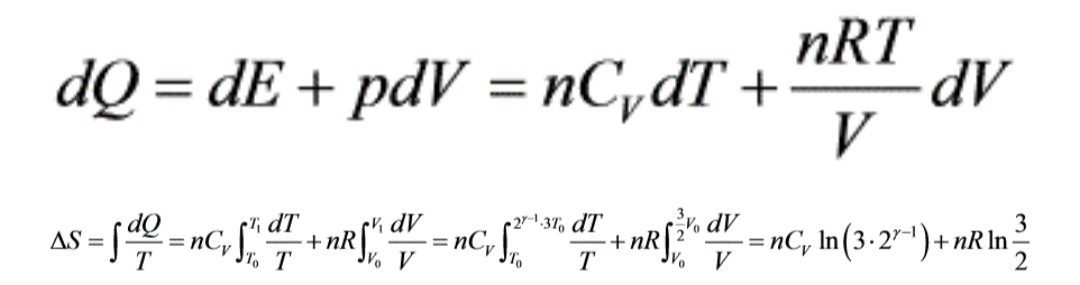
\includegraphics[width=1\linewidth]{Screenshot_20250416_201806.jpg}
    \end{figure}
\end{enumerate}




\subsection*{2.5}

\subsubsection*{对于第(1)问的解答如下:}

---

\paragraph*{单缝衍射中央明条纹线宽度的计算}

---

\subparagraph*{公式推导} \mbox{} \\

单缝衍射的中央明纹线宽度 \(\Delta x_0\) 定义为两个第一级暗纹之间的距离。根据单缝衍射暗纹条件:  
\[
a \sin\theta = \pm \lambda \quad (k=1)
\]  
中央明纹的角宽度为 \(2\theta\),对应的线宽度为:  
\[
\Delta x_0 = 2 \cdot f \cdot \tan\theta \approx 2 \cdot f \cdot \sin\theta \quad (\text{小角度近似})
\]  
代入暗纹条件 \(\sin\theta = \frac{\lambda}{a}\),得:  
\[
\Delta x_0 = 2 \cdot f \cdot \frac{\lambda}{a}
\]

---

\subparagraph*{代入数据} \mbox{} \\

已知:  
\begin{itemize}
    \item 缝宽 \(a = 6 \times 10^{-6} \, \text{m}\)  
    \item 波长 \(\lambda = 600 \, \text{nm} = 600 \times 10^{-9} \, \text{m}\)  
    \item 焦距 \(f = 1.5 \, \text{m}\)  
\end{itemize}

代入公式计算:  
\[
\Delta x_0 = 2 \cdot 1.5 \cdot \frac{600 \times 10^{-9}}{6 \times 10^{-6}} = 2 \cdot 1.5 \cdot 0.1 = 0.3 \, \text{m} = 30 \, \text{cm}
\]

---

\subparagraph*{关键验证}

\begin{itemize}
    \item \textbf{量纲检查}:分子为 \([f \cdot \lambda] = \text{m} \cdot \text{m}\),分母为 \([a] = \text{m}\),最终量纲为 \(\text{m}\),符合物理意义。  
    \item \textbf{数值合理性}:  
    \begin{itemize}
        \item 光波长与缝宽比例 \(\frac{\lambda}{a} = \frac{600 \, \text{nm}}{6 \, \mu\text{m}} = 0.1\),对应衍射显著。  
        \item 透镜焦距 \(1.5 \, \text{m}\) 导致明纹宽度较大(30 cm),与实际实验现象一致。
    \end{itemize}
\end{itemize}

---

\subparagraph*{最终答案}

单缝衍射中央明条纹的线宽度为:  
\[
\boxed{\Delta x_0 = 0.3 \, \text{m} \, \text{(或 } 30 \, \text{cm)}}
\]

\subsubsection*{对于第(2)问的解答如下:}

---

\paragraph*{光栅主极大级次的分析}

---

\subparagraph*{1. 光栅常数与主极大位置}

\begin{itemize}
    \item 光栅常数 \( d = \frac{1 \, \text{cm}}{500} = 2 \times 10^{-5} \, \text{m} \)。  
    \item 光栅主极大的位置由光栅方程 \( d \sin\theta = k\lambda \) 决定,在透镜焦平面上的坐标为:  
    \[
    x_k \approx f \cdot \tan\theta \approx f \cdot \frac{k\lambda}{d}
    \]
\end{itemize}

---

\subparagraph*{2. 主极大在 \(\Delta x_0\) 内的条件} \mbox{} \\
\begin{figure}[H]
    \centering
    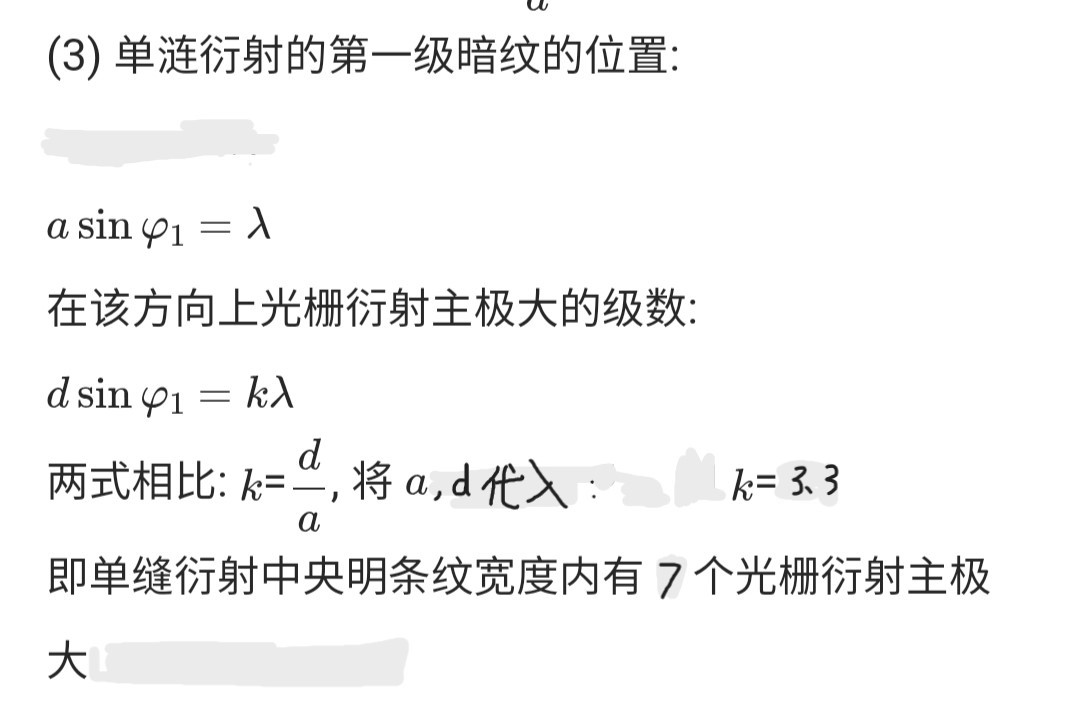
\includegraphics[width=1\linewidth]{Screenshot_20250416_204332.jpg}
\end{figure}
单缝衍射中央明纹的线宽度 \(\Delta x_0 = 0.3 \, \text{m}\),主极大需满足:  
\[
|x_k| \leq \frac{\Delta x_0}{2} = 0.15 \, \text{m}
\]  
代入 \( x_k \) 表达式:  
\[
\left| \frac{k \lambda f}{d} \right| \leq 0.15 \implies |k| \leq \frac{0.15 \cdot d}{\lambda f}
\]

---

\subparagraph*{3. 最大级次计算} \mbox{} \\

代入已知值:  
\[
k_{\text{max}} = \frac{0.15 \cdot 2 \times 10^{-5}}{600 \times 10^{-9} \cdot 1.5} = \frac{3 \times 10^{-6}}{9 \times 10^{-7}} \approx 3.33
\]  
由于 \( k \) 必须为整数,因此最大级次为 \( k = \pm 3 \)。

---

\subparagraph*{4. 可能的级次} \mbox{} \\

在 \(\Delta x_0\) 范围内,可观察到的光栅主极大级次为:  
\[
k = 0, \pm 1, \pm 2, \pm 3
\]

---

\paragraph*{关键验证}

\begin{itemize}
    \item \textbf{k=3 的位置}:  
    \[
    x_3 = \frac{3 \cdot 600 \times 10^{-9} \cdot 1.5}{2 \times 10^{-5}} = 0.135 \, \text{m} < 0.15 \, \text{m}
    \]  
    在 \(\Delta x_0\) 内。  
    \item \textbf{k=4 的位置}:  
    \[
    x_4 = \frac{4 \cdot 600 \times 10^{-9} \cdot 1.5}{2 \times 10^{-5}} = 0.18 \, \text{m} > 0.15 \, \text{m}
    \]  
    超出范围。
\end{itemize}

---

\paragraph*{最终答案} \mbox{} \\

在单缝衍射中央明条纹的线宽度 \(\Delta x_0\) 内,可能观察到的光栅衍射主极大的级次为:  
\[
\boxed{k = 0, \pm 1, \pm 2, \pm 3}
\]

\subsubsection*{对于第(3)问的解答如下:}

---

\paragraph*{缺级现象的最小级次分析}

---

\subparagraph*{1. 缺级条件} \mbox{} \\

缺级发生在多缝干涉主极大与单缝衍射极小位置重合时,即满足:  
\[
\begin{cases}
\text{光栅方程:} & d \sin\theta = k\lambda \quad (k \in \mathbb{Z}) \\
\text{单缝衍射极小条件:} & a \sin\theta = m\lambda \quad (m \in \mathbb{Z}^+)
\end{cases}
\]  
联立两式得:  
\[
k = \frac{d}{a} \cdot m
\]  
其中 \( \frac{d}{a} \) 必须为有理数,且 \( k \) 需为整数。

---

\subparagraph*{2. 参数计算}

\begin{itemize}
    \item \textbf{光栅常数}:  
    \[
    d = \frac{1 \, \text{cm}}{500} = \frac{0.01 \, \text{m}}{500} = 2 \times 10^{-5} \, \text{m}
    \]  
    \item \textbf{缝宽}:  
    \[
    a = 6 \times 10^{-6} \, \text{m}
    \]  
    \item \textbf{比值}:  
    \[
    \frac{d}{a} = \frac{2 \times 10^{-5}}{6 \times 10^{-6}} = \frac{10}{3} \quad (\text{化简为互质分数})
    \]
\end{itemize}

---

\subparagraph*{3. 最小缺级级次} \mbox{} \\

当 \( \frac{d}{a} = \frac{10}{3} \)(分子分母互质),最小缺级级次为:  
\[
k = \frac{10}{3} \cdot m \quad \implies \quad m = 3 \quad \text{时,} \quad k = 10
\]  
\textbf{结论}:缺级的最小级次为 \( k = 10 \)。

---

\paragraph*{验证与物理意义}

\begin{itemize}
    \item \textbf{k=10 的主极大位置}:  
    \[
    \sin\theta = \frac{10 \lambda}{d} = \frac{10 \cdot 600 \times 10^{-9}}{2 \times 10^{-5}} = 0.3 \quad (\theta \approx 17.46^\circ)
    \]  
    \item \textbf{对应的单缝衍射极小级次}:  
    \[
    m = \frac{a \sin\theta}{\lambda} = \frac{6 \times 10^{-6} \cdot 0.3}{600 \times 10^{-9}} = 3
    \]  
    满足 \( m=3 \),单缝衍射第3级极小与多缝干涉第10级主极大重合,导致缺级。
\end{itemize}

---

\paragraph*{最终答案} \mbox{} \\

出现缺级现象的最小级次为:  
\[
\boxed{k = 10}
\]
\subsubsection*{对于第(4)问的解答如下:}

---

\paragraph*{光栅分辨率与总缝数的计算}

---

\subparagraph*{1. 分辨率公式} \mbox{} \\

光栅的分辨本领 \( R \) 定义为:  
\[
R = \frac{\lambda}{\Delta\lambda} = k \cdot N
\]  
其中:  
• \( k \) 为主极大级次(题目中为第二主极大,即 \( k = 2 \)),  
• \( N \) 为光栅总缝数,  
• \( \Delta\lambda = 0.005 \, \text{nm} \) 为可分辨的最小波长差。

---

\subparagraph*{2. 代入已知数据} \mbox{} \\

已知 \( \lambda = 600 \, \text{nm} \),\( \Delta\lambda = 0.005 \, \text{nm} \),代入公式:  
\[
R = \frac{600}{0.005} = 120,000
\]  
由 \( R = k \cdot N \),得:  
\[
N = \frac{R}{k} = \frac{120,000}{2} = 60,000
\]

---

\subparagraph*{3. 物理意义验证} \mbox{} \\

\begin{itemize}
    \item \textbf{总缝数合理性}:光栅每厘米有 \( 500 \) 条缝,总缝数 \( N = 60,000 \) 对应的光栅长度为:  
    \[
    L = \frac{N}{500} \, \text{cm} = 120 \, \text{cm} = 1.2 \, \text{m}  
    \]  
    长度合理(常见光栅尺寸为分米至米量级)。  
    \item \textbf{分辨率要求}:高分辨率光栅需要大缝数 \( N \),与计算结果一致。
\end{itemize}

---

\paragraph*{最终答案} \mbox{} \\

光栅的总缝数为:  
\[
\boxed{N = 60,000}
\]

\newpage
\section*{2021}



\newpage
\section*{2022}





\end{document}